\documentclass[11pt]{article}
\usepackage{theme}
\usepackage{shortcuts}
\usepackage{subcaption}
% Document parameters
% Document title
\title{Projet final (ML for TS) - MVA 2023/2024}
\author{
Inès Vati \email{ines.vati@eleves.enpc.fr} \\ % student 1
Mathis Reymond \email{mathis.reymond74@gmail.com} % student 2
}

\begin{document}
\maketitle

\section{Introduction}

\section{Principe du \textit{Graph Signal Processing}}
\subsection{Graph Fourier Transform}

L'article introduit une transformée de Fourier sur les graphes. Pour définir cette transformée sur un graphe $G$, il faut choisir une représentation matricielle $S$ de cette matrice (généralement matrice d'adjacence ou Laplacienne, mais d'autres matrices peuvent être envisagées). Il faut ensuite diagonaliser cette matrice et l'écrire sous la forme
\begin{align}
    S = V\Lambda V^{-1}
\end{align}
où $\Lambda$ est une matrice diagonale contenant les valeurs propres de $S$ et $V$ une matrice de veceurs propres associée. Cela permet alors de définir, étant donnée un signal $x$ sur $G$, la transformée de Fourier de $x$ sur $G$ par
\begin{equation}
    \Tilde{x} := V^Tx \label{eq:GFT}
\end{equation}
Pour développer l'intuition, et voir plus clairement le parallèle avec la transformée de Fourier discrète, il peut être intéressant de se demander si un graphe permet de retrouver l'interprétation habituelle de la transformée de Fourier discrète d'un signal temporel. Les graphes cycliques permettent cela. En effet, soit un signal $x$ sur le graphe cycle à $N$ sommets $C_N$. La matrice d'adjacence $H_N$ de ce graphe est 
\[ A_N := 
\begin{bmatrix}
0 & 1 & 0 & 0 & 0 & 1 \\
1 & 0 & 1 & 0 & 0 & 0 \\
0 & 1 & 0 & 1 & 0 & 0 \\
0 & 0 & 1 & 0 & 1 & 0 \\
0 & 0 & 0 & 1 & 0 & 1 \\
1 & 0 & 0 & 0 & 1 & 0 \\
\end{bmatrix}
\]
En notant
\[J :=
\begin{bmatrix}
0 & 1 & 0 & \dots & 0 \\
0 & 0 & 1 & \dots & 0 \\
\vdots  &     &     & \ddots & \vdots  \\
0 & & &        & 1 \\
1 & 0 & 0 & \dots  & 0
\end{bmatrix}
\]
on observe que 
\begin{align}
    A_N = J + j^{N-1}
\end{align}
Or les valeurs propres de $J$ sont les racines $N$-ièmes de l'unité $\omega^0,...,\omega^{N-1}$ où $\omega := e^{\frac{2i\pi}{n}}$ et pour tout $k\in [\![0,N-1]\!]$, \[X_k := \begin{bmatrix} 1 \\\omega^k \\ \omega^{2k}\\ \vdots\\ \omega^{(n-1)k}\end{bmatrix}\]
est vecteur propre de $J$ associé à la valeur propre $\omega^k$.
Cela permet donc, en notant $W$ la matrice de transformée de Fourier discète
\[ W :=
\begin{bmatrix}
1&1&1&1&\cdots &1 \\
1&\omega&\omega^2&\omega^3&\cdots&\omega^{N-1} \\
1&\omega^2&\omega^4&\omega^6&\cdots&\omega^{2(N-1)}\\ 1&\omega^3&\omega^6&\omega^9&\cdots&\omega^{3(N-1)}\\
\vdots&\vdots&\vdots&\vdots&\ddots&\vdots\\
1&\omega^{N-1}&\omega^{2(N-1)}&\omega^{3(N-1)}&\cdots&\omega^{(N-1)(N-1)}
\end{bmatrix}
\]
d'écrire
\begin{align}
    A_N = W(\Omega+\Omega^{N-1})W^{-1}
\end{align}
où $\Omega := Diag(w^0,...,w^{N-1})$\\
Ainsi, les valeurs propres de $A_N$ sont donc les $\lambda_k = \omega^k+\omega^{n-k}$ pour $k \in [\![0,N-1]\!]$.\\
En utilisant la définition de la transformée de Fourier sur les graphes \ref{eq:GFT}, on explicite le $k$-ième coefficient de Fourier
\begin{align}
    \Tilde{x}_k &= W_k^Tx\\
    &= \sum_{n=0}^{N-1}x_n\omega^{nk} \\
    &= \sum_{n=0}^{N-1}x_n e^{2i\pi n\frac{k}{N}}
\end{align}

\begin{figure}[h]
  \centering
  \begin{subfigure}{0.35\linewidth}
    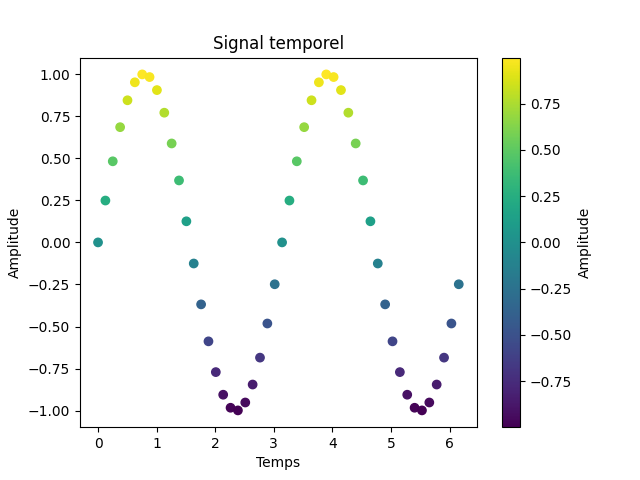
\includegraphics[width=6.5cm]{img/temporal_signal.png}
    \caption{Représentation temporelle d'un signal echantillonné}
    \label{fig:DANN_1}
  \end{subfigure}
  \hspace{1.5cm}
  \begin{subfigure}{0.35\linewidth}
    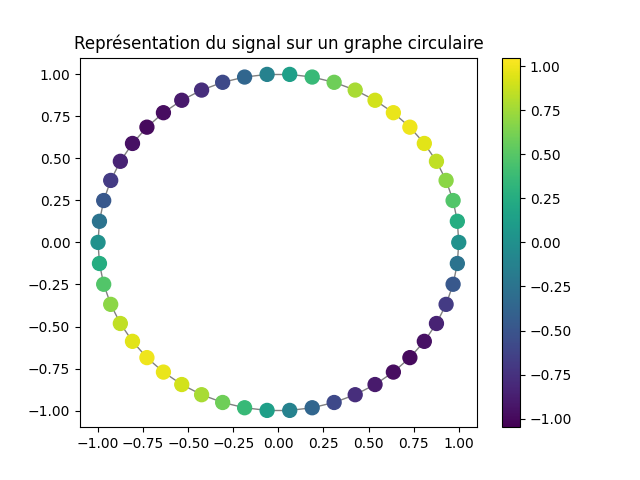
\includegraphics[width=6.5cm]{img/graph_signal.png}
    \caption{Représentation du même signal sur un graphe circulaire}
    \label{fig:DANN_2}
  \end{subfigure}
  \caption{Deux représentations d'un signal échantillonné dont on calcule la transformée de Fourier par les deux définitions dont on dispose : la transformée de Fourier discrète, et la transformée de Fourier d'un graphe}
  \label{fig:DANN}
\end{figure}

\subsection{Graph Filtering}

\subsection{Graph Surrogate Signal}

\section{Expériences}

\subsection{Dataset BOLD5000}


\section{Conclusion et Discussion}

\end{document}
